%!TEX program = xelatex
% 完整编译: xelatex -> biber/bibtex -> xelatex -> xelatex
\documentclass[lang=en,11pt,a4paper]{elegantpaper}

\title{FEM for the 2D convection-diffusion equation}
\author{W Huang}


% 本文档命令
\usepackage{array}
\usepackage{float}
\usepackage{multirow}
\newcommand{\ccr}[1]{\makecell{{\color{#1}\rule{1cm}{1cm}}}}

\begin{document}

\maketitle

\section{Formulas}

We want to solve the 2D convection-diffusion equation
\begin{equation}
    \frac{\partial \mathbf{u}}{\partial t}=-(\mathbf{u}\cdot \nabla)\mathbf{u}+\mathbf{g}+\nu \Delta \mathbf{u}.
\end{equation}

The IMEX-trapezoidal RK method gives the time discretization
\begin{align}
    \left(1-\frac{1}{2}k\nu\Delta\right)\mathbf{u}^*&=\mathbf{u}^{n}+\frac{1}{2}k\nu\Delta\mathbf{u}^{n}-k(\mathbf{u}^n\cdot \nabla)\mathbf{u}^n+k\mathbf{g}^n,\\
    \mathbf{u}^{**}&=\frac{1}{2}(\mathbf{u}^n+\mathbf{u}^*),\\
    \mathbf{u}^{n+1}&=\mathbf{u}^n+k\nu\Delta\mathbf{u}^{**}-k(\mathbf{u}^{**}\cdot \nabla)\mathbf{u}^{**}+\frac{k}{2}(\mathbf{g}^n+\mathbf{g}^{n+1}).
\end{align}

The only challenge is the convection terms $(\mathbf{u}\cdot \nabla)\mathbf{u}$. 
The FEM discretization gives that
\begin{align}
    u_1^n&=\sum_{j=1}^N U_{1,j}^n \Phi_j,\\
    u_2^n&=\sum_{j=1}^N U_{2,j}^n \Phi_j.
\end{align}

Inner-product the convection terms with the test function $\Phi_i$, we have, for example
\begin{align}
    \left(u_1^n\frac{\partial u_1^n}{\partial x}, \Phi_i\right)&=\sum_{j,k=1}^N U_{1,j}^n U_{1,k}^n \left(\Phi_j\frac{\partial \Phi_k}{\partial x}, \Phi_i\right)\\
    &= \sum_{q=1}^Q \sum_{j,k=1}^N U_{1,j}^n U_{1,k}^n \Phi_j(v_q)\frac{\partial \Phi_k}{\partial x}(v_q)\Phi_i(v_q) w_q\\
    &= \sum_{q=1}^Q w_q\Phi_i(v_q) \left(\sum_{j=1}^N U_{1,j}^n\Phi_j(v_q)\right) \left(\sum_{k=1}^N U_{1,k}^n\frac{\partial \Phi_k}{\partial x}(v_q)\right).
\end{align}

Similar for other convection terms. So the $(q,i,j,k)$-loop is reduced to $(q,i)$-loops. 
The summation shall not write in hand. 
Instead, \verb|deal.ii| provided functions \verb|get_function_values| and \verb|get_function_gradients|
to do such work.

Note that if we use the $Q_k$ element, a quadrature formula with algebraical accuracy of order at 
least $(3k-1)$ is required. For example, the $Q_1$ element needs the $2$-points Gauss quadrature formula.

\section{Numerical experiments}

In this sectoin, we test our program with the conditions derived from the exact solution, 
a divergence-free velocity field with a single vortex,
\begin{equation}
    \mathbf{u}(x,y)=\cos\frac{\pi t}{T}(\sin^2(\pi x)\sin(2\pi y),-\sin(2\pi x)\sin^2(\pi y)),
\end{equation}
where $T$ could be any positive real number, for example, $1$.

The domain boundary conditions are homogeneous Dirichlet. The forcing terms are
\begin{align}
    g_1(x,y) =& -\frac{\pi}{T}\sin\frac{\pi t}{T} \sin^2(\pi x) \sin(2\pi y) \nonumber \\
              & + \pi\cos^2\frac{\pi t}{T}\sin^2(\pi x)\sin(2\pi x)\sin^2(2\pi y) \nonumber \\
              & - 2\pi\cos^2\frac{\pi t}{T}\sin(2\pi x)\sin^2(\pi x)\sin^2(\pi y)\cos(2\pi y) \nonumber \\
              & - 2\pi^2\nu \cos\frac{\pi t}{T}\cos(2\pi x)\sin(2\pi y) \nonumber \\
              & + 4\pi^2\nu \cos\frac{\pi t}{T}\sin^2(\pi x)\sin(2\pi y),\\
    g_2(x,y) =& \frac{\pi}{T}\sin\frac{\pi t}{T} \sin(2\pi x) \sin^2(\pi y) \nonumber \\
              & + \pi\cos^2\frac{\pi t}{T}\sin^2(\pi y)\sin(2\pi y)\sin^2(2\pi x) \nonumber \\
              & - 2\pi\cos^2\frac{\pi t}{T}\sin(2\pi y)\sin^2(\pi y)\sin^2(\pi x)\cos(2\pi x) \nonumber \\
              & + 2\pi^2\nu \cos\frac{\pi t}{T}\cos(2\pi y)\sin(2\pi x) \nonumber \\
              & - 4\pi^2\nu \cos\frac{\pi t}{T}\sin^2(\pi y)\sin(2\pi x).
\end{align}

The vorticity changes its sign at $t=\frac{T}{2}$, see the following figures.
\begin{figure}[H]
    \centering
    \begin{minipage}[t]{0.4\linewidth}
        \centering
        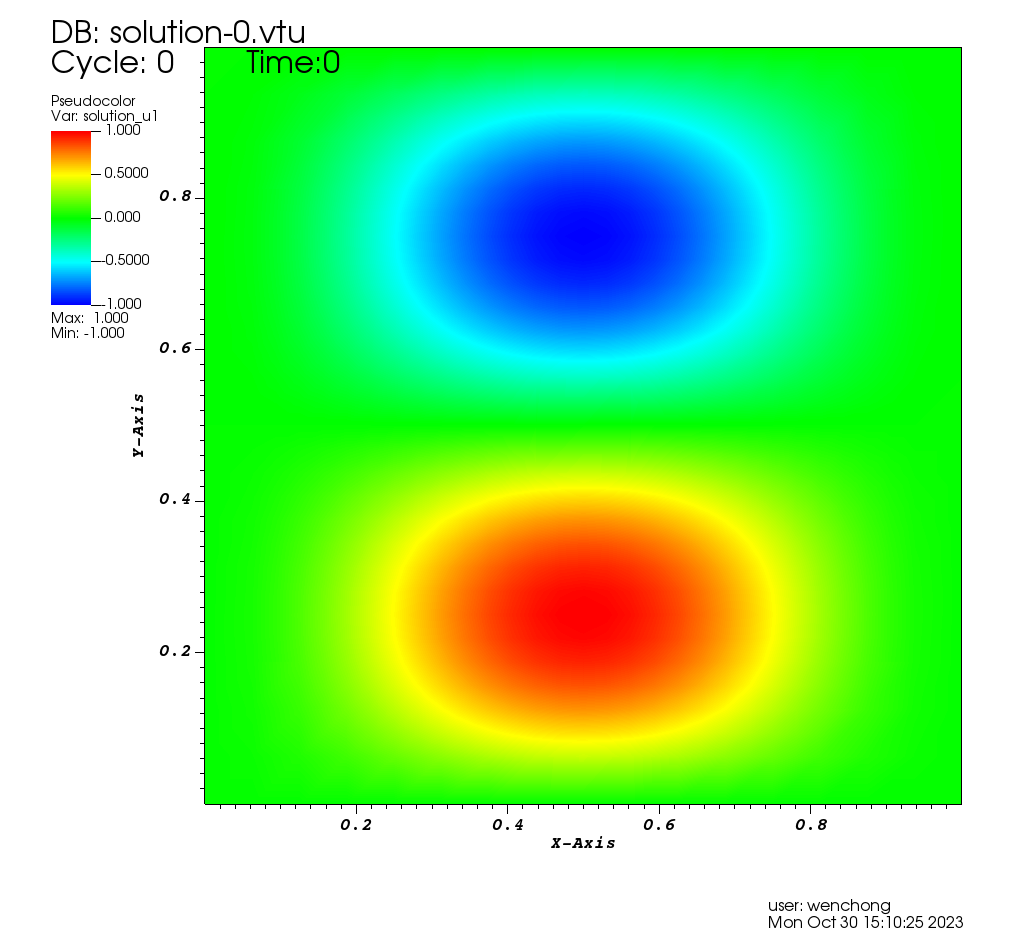
\includegraphics[width=0.8\linewidth]{png/ux_t=0.png}
        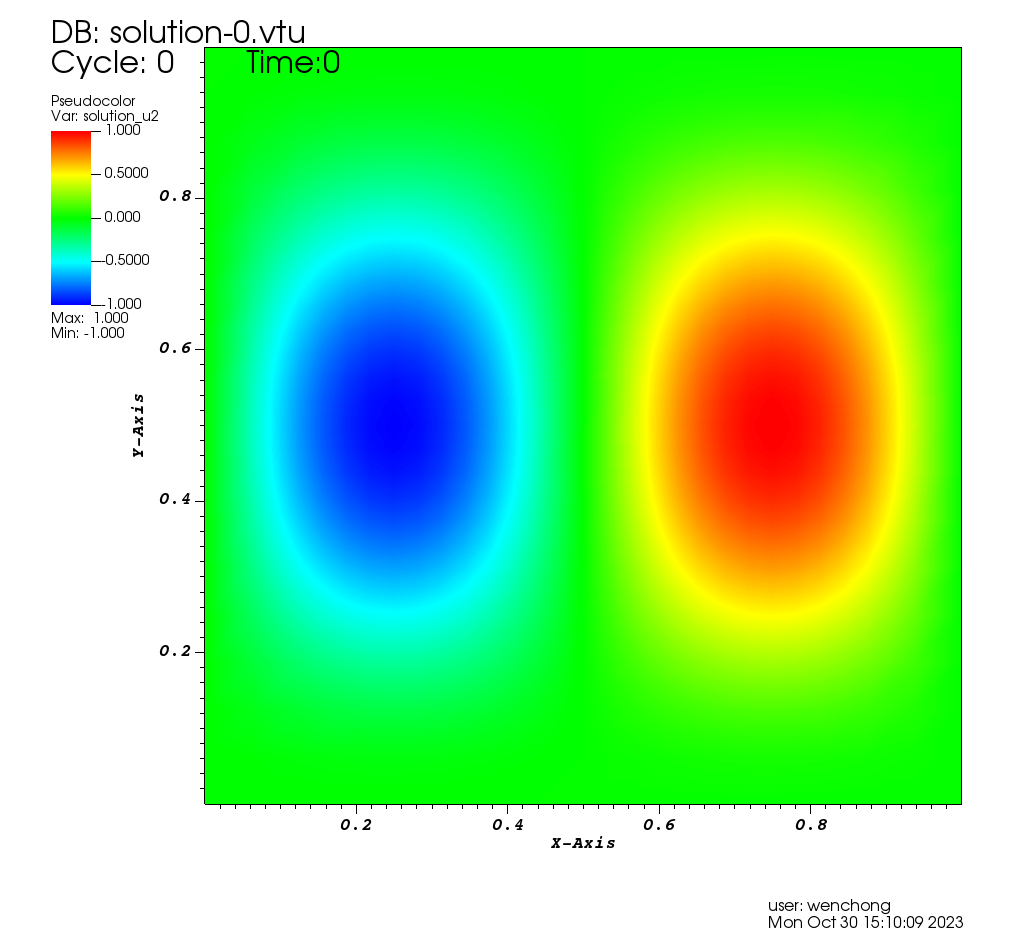
\includegraphics[width=0.8\linewidth]{png/uy_t=0.png}
        \caption*{\small $u_1,u_2$ at $t=0$.}
    \end{minipage}
    \begin{minipage}[t]{0.4\linewidth}
        \centering
        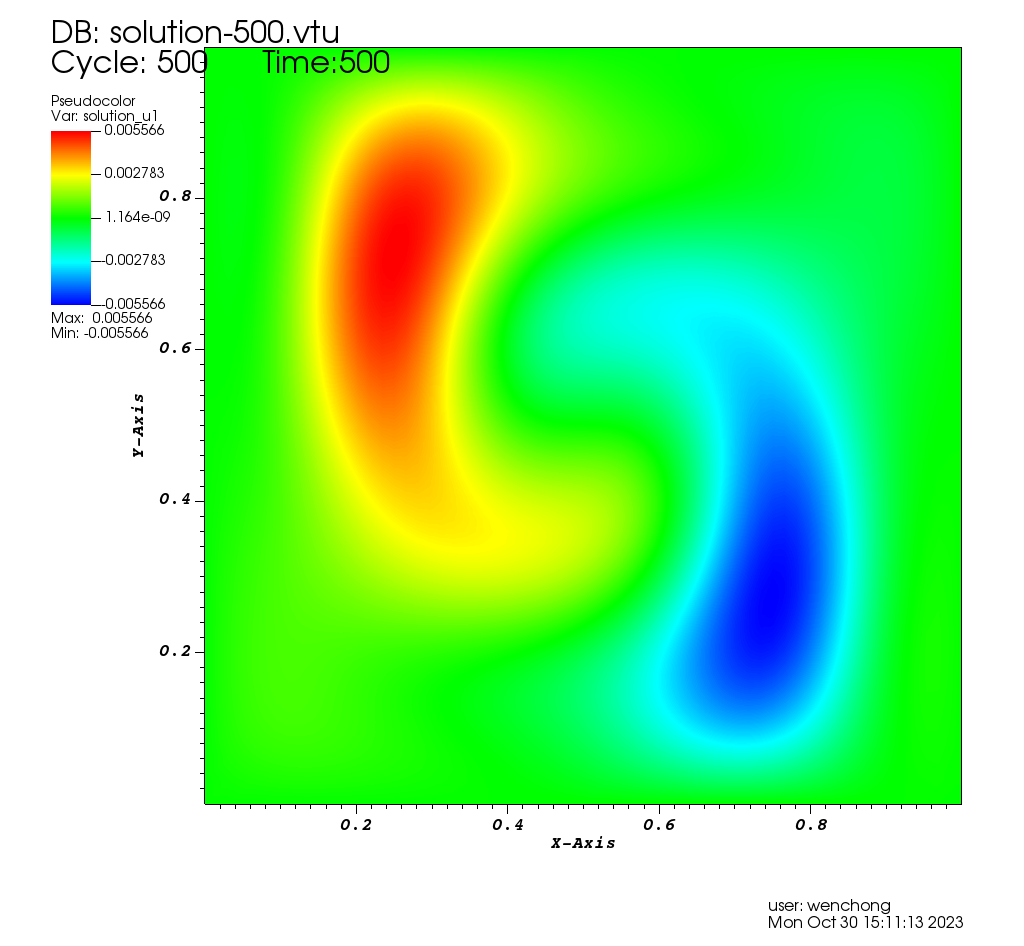
\includegraphics[width=0.8\linewidth]{png/ux_t=0.5.png}
        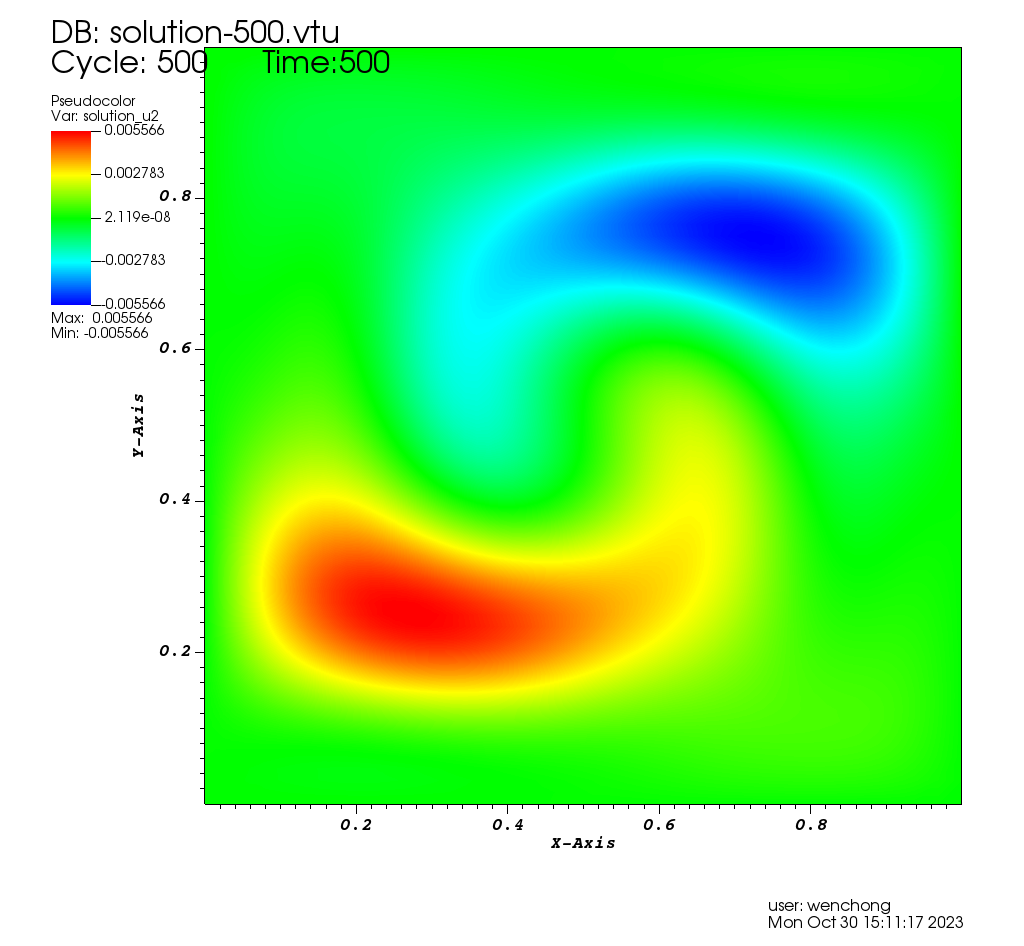
\includegraphics[width=0.8\linewidth]{png/uy_t=0.5.png}
        \caption*{\small $u_1,u_2$ at $t=\frac{T}{2}$.}
    \end{minipage}
\end{figure}

We use an adaptive mesh with width $h,\frac{h}{2},\frac{h}{4},\frac{h}{8}$. 
But the error distribution is so uniform that the adaptive mesh looks useless.
\begin{figure}[H]
    \centering
    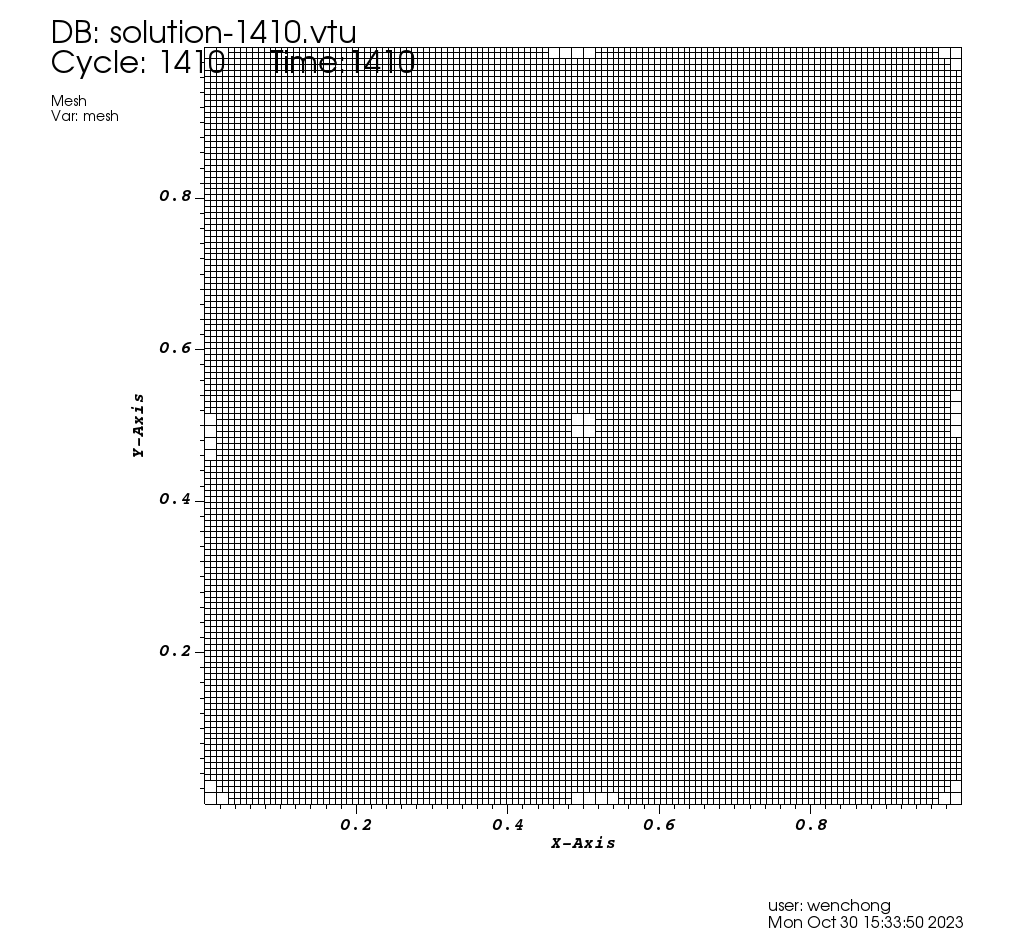
\includegraphics[width=0.5\linewidth]{png/mesh.png}
    \caption*{\small Adaptive mesh, $h=\frac{1}{8}$.}
\end{figure}

\begin{figure}[H]
    \centering
    \begin{minipage}[t]{0.4\linewidth}
        \centering
        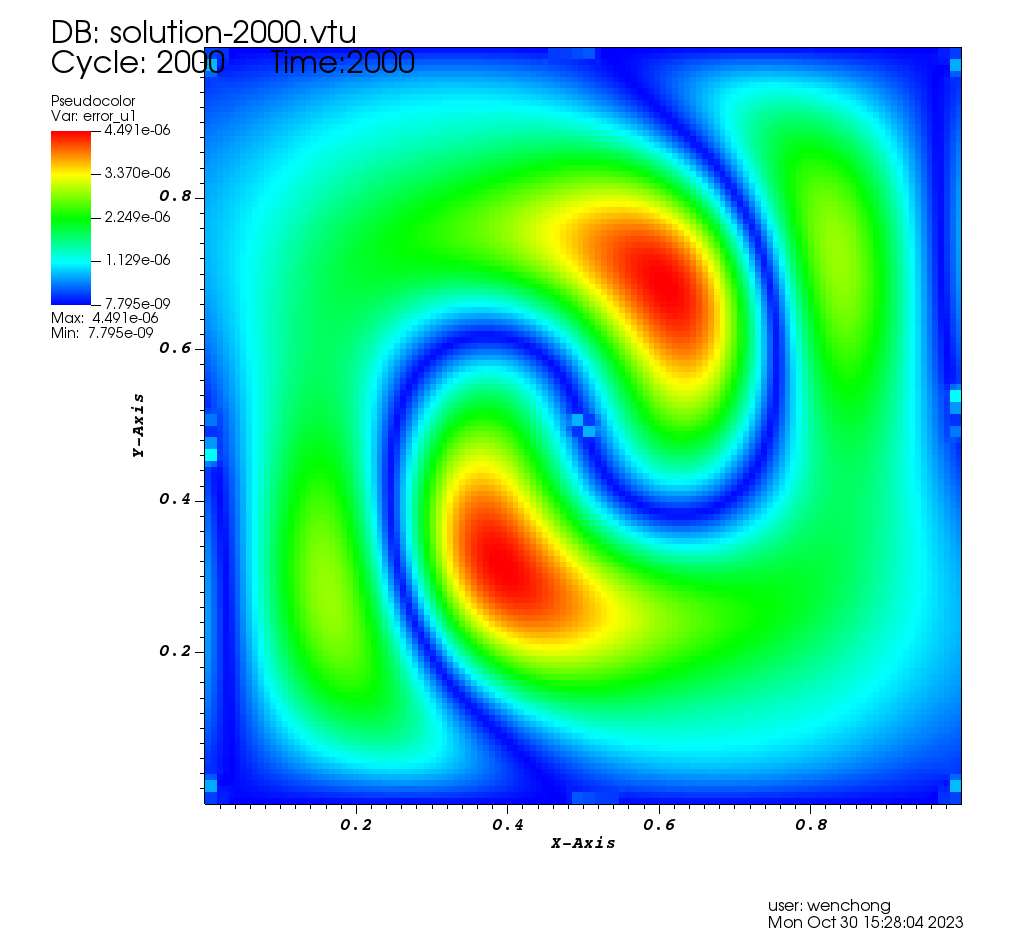
\includegraphics[width=0.8\linewidth]{png/err_ux_t=1.png}
        \caption*{\small Error distribution of $u_1$, $t=T$, $h=\frac{1}{8}$.}
    \end{minipage}
    \begin{minipage}[t]{0.4\linewidth}
        \centering
        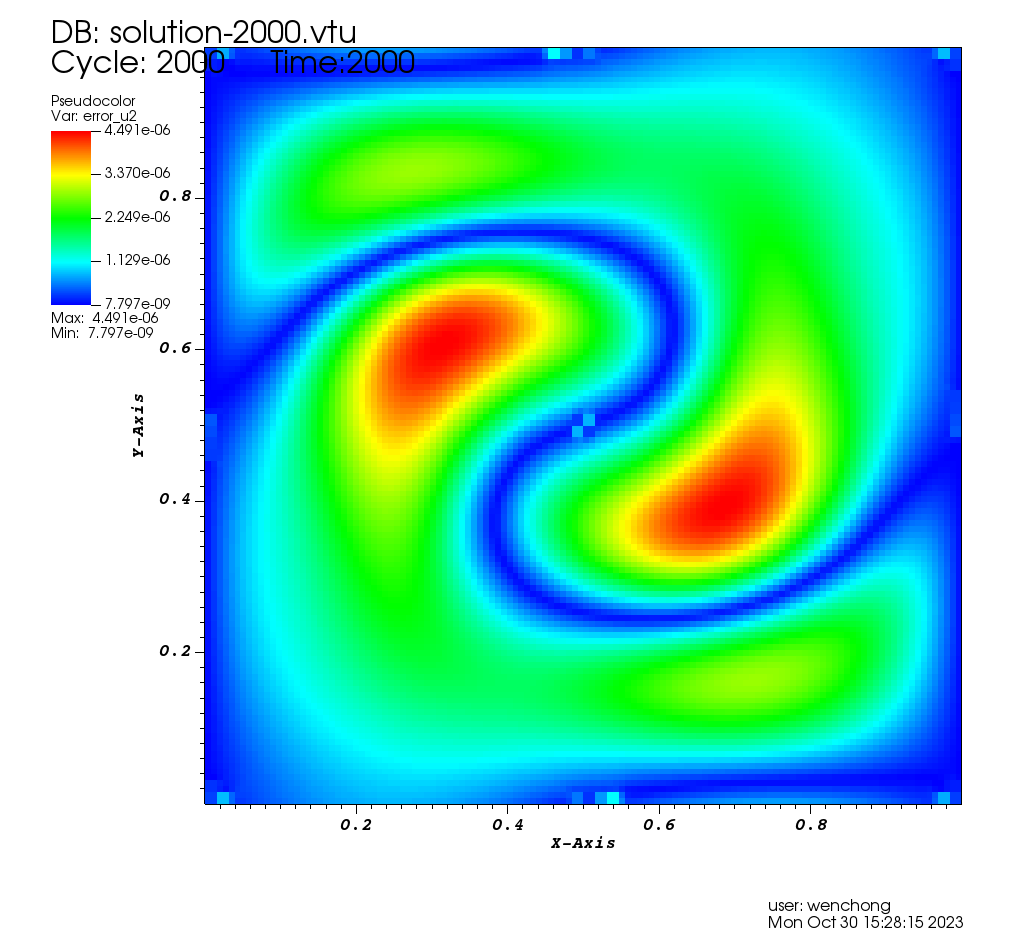
\includegraphics[width=0.8\linewidth]{png/err_uy_t=1.png}
        \caption*{\small Error distribution of $u_1$, $t=T$, $h=\frac{1}{8}$.}
    \end{minipage}
\end{figure}

We choose the $Q_1$ element. And the time step is $\frac{h}{250}$. 
Here is the convergence table. 
The $2$-nd order convergence rate of the $L_2$ norm is valid.
It is interesting that the errors decrease over time.

\begin{table}[H]
    \centering
    \begin{tabular}{cccccc}
    \hline
    $h$                                    & $\frac{1}{4}$ & Rate & $\frac{1}{8}$ & Rate & $\frac{1}{16}$ \\ \hline
    $||u^h_1-u_1||_{L_2}$, $t=\frac{T}{2}$ & 0.00211047    & 1.99 & 0.000531287   & 2.01 & 0.000132154    \\
    $||u^h_2-u_2||_{L_2}$, $t=\frac{T}{2}$ & 0.00211048    & 1.99 & 0.000531294   & 2.01 & 0.000132157    \\ \hline
    $||u^h_1-u_1||_{L_2}$, $t=T$           & 0.000925229   & 1.99 & 0.000232991   & 2.02 & 5.76028e-05    \\
    $||u^h_2-u_2||_{L_2}$, $t=T$           & 0.000925245   & 1.99 & 0.000232999   & 2.02 & 5.76034e-05    \\ \hline
    \end{tabular}
\end{table}

\appendix
%\appendixpage
\addappheadtotoc

\end{document}
